Afin d'héberger Clever Party Thrower, plusieurs possibilités s'offrent au client.
Celles-ci dépendent de son budget, de l'infrastructure dont il dispose et du nombre d'utilisateurs qui devront être servis.

\subsection{docker-compose}\label{subsec:docker-compose}
L'application, étant packagée dans des conteneurs Docker, peut être déployée très facilement dans un environnement restreint grâce à Docker et Docker Compose.
Durant le développement de l'application, j'ai souhaité permettre à des utilisateurs potentiels du service de tester certaines parties de l'interface.\\

J'ai donc décidé d'héberger un stack Docker Compose sur un petit serveur de mon homelab.
Le stack que j'ai choisi de décrire dans la documentation est minimaliste, il comprend le strict nécessaire pour héberger et utiliser l'application.
Le fichier docker-compose comprend le backend, la base de données et le frontend hébergé par un serveur nginx.

\subsection{kubernetes}\label{subsec:kubernetes}
Lorsque le client dispose d'une infrastructure performante, il a la possibilité de déployer l'application sur un ou plusieurs clusters Kubernetes.
Durant le développement de l'application, je me suis intéressé à l'orchestration de conteneurs avec Kubernetes,
ce qui m'a conduit à proposer des fichiers de configuration pour héberger le site web et son serveur.\\

En parallèle de ma formation sur Kubernetes, j'ai également exploré Ansible et ai adapté un projet open-source existant afin de permettre le déploiement de Clever Party Thrower sur un cluster Kubernetes en une seule commande.
Ce playbook Ansible facilite le déploiement d'un cluster K3S complet, avec ou sans haute disponibilité.
De plus, le playbook déploie également des applications telles que kubeVip, MetalLB, Rancher, Traefik, Cert-manager, LongHorn et ArgoCD.

\subsubsection{Le Playbook}
Le Playbook permet de déployer Kubernetes sur plusieurs machines, appelées nodes, afin d'ajouter de la résilience au cluster.
Plus il y a de nodes, plus le cluster peut en perdre sans interruption de service.
Les différentes applications utilisées pour permettre cette haute disponibilité sont les suivantes : \\

\begin{itemize}
    \item \textbf{Kubernetes} : Kubernetes synchronise et répartit toutes les configurations et les ressources entre les différentes nodes
    pour garantir que chacune d'entre elles peut à tout moment gérer le trafic.\\

    \item \textbf{Kubevip} : Kubevip sert à créer une adresse virtuelle pour la gestion du cluster.
    Cette adresse virtuelle permet de conserver une connexion avec le cluster tant qu'au moins une des nodes master est en ligne et fonctionnelle .\\

    \item \textbf{MetalLB} : MetalLB est un load balancer qui, comme son nom l'indique, permet d'équilibrer la charge de travail.
    Il attribue également des adresses IP à des pods (conteneurs dans Kubernetes) en fonction de leur nom ou espace de nom et ce, dans une plage définie .\\

    \item \textbf{Cert-manager} : Cert-manager permet de créer et renouveler les différents certificats via Let's Encrypt,
    en plus de permettre à Kubernetes de les gérer comme toute autre ressource, et donc de les synchroniser entre les différentes nodes.\\


    \item \textbf{Traefik} : Traefik sert de reverse proxy, protégeant ainsi les différents services du cluster.
    Il gère également la distribution de la charge pour les requêtes \Gls{https} .\\
    \item \textbf{Longhorn} : Longhorn permet de créer des volumes partagés et disponibles sur plusieurs nodes en même temps,
    garantissant ainsi aux pods exploitant ces volumes qu'ils seront toujours accessibles.\\
\end{itemize}

\subsection{Les Conteneurs}\label{subsec:les-conteneurs}
Le conteneur back-end est relativement simple.
Il utilise une image node:latest.
Une fois le code source transpilé, le résultat de cette compilation est copié dans l'image.\\

Le conteneur pour la base de données utilise quant à lui une simple image de PostGIS.
PostGIS est une extension de PostgreSQL qui permet la manipulation de points géographiques directement sur la base de données.\\

Le conteneur front-end est plus complexe.
Basé sur une image nginx, il intègre le résultat de la compilation Angular dans le dossier où nginx cherche les fichiers à servir.
Nginx sert donc le front end, et agit également comme un proxy pour permettre au front end d'accéder au backend.

\subsection{Mon choix}\label{subsec:mon-choix}
En tant que client, j'ai choisi d'héberger l'application via docker-compose.\\

À l'origine, mon objectif était de créer un cluster Kubernetes distribué entre plusieurs machines virtuelles pour simuler
diverses machines physiques, et de déployer l'application sur ce cluster.
Cependant, Kubernetes, et surtout la haute disponibilité, exige beaucoup de ressources, que mon serveur ne pouvait pas supporter.
Les différentes machines virtuelles manquaient constamment de mémoire ou d'espace disque.\\

J'ai ainsi décidé d'utiliser un simple docker-compose pour optimiser les ressources de mon serveur,
permettant d'héberger toutes mes applications plutôt que de se limiter à une seule avec des performances médiocres.
À l'avenir, si les limites matérielles ne sont plus un obstacle, j'envisagerai de déployer une infrastructure Kubernetes via Ansible,
avec l'ajout d'un système de surveillance.

\subsection{Sécurité et hébergement}\label{subsec:securite-et-hebergement}
Étant donné que le client est potentiellement responsable de l'hébergement de l'application, une grande partie des
responsabilités en termes de sécurité lui revient.
L'application doit être hébergée derrière un reverse proxy pour assurer la terminaison SSL, par exemple.
Les deux différentes méthodes d'hébergement assurent la sécurité de la base de données via le réseau Docker : seul le backend
a accès à la base de données.\\

Les différentes applications sont maintenues à jour soit via ArgoCD sur Kubernetes, soit via Watchtower sur Docker Compose.
Ces deux applications surveillent l'état du dépôt Docker Hub en temps réel et mettent à jour les services lors d'un changement.\\

Pour mon installation, j'ai choisi de faire confiance à Cloudflare pour sécuriser mon hébergement.
J'utilise un tunnel et leur reverse proxy afin de garantir la sécurité de mes services.
Cloudflare gère non seulement les certificats, mais permet aussi de bloquer les attaques de type DDoS. De plus, grâce au tunnel,
je n'ai pas à configurer mon pare-feu sur mon router ni à exposer mon adresse IP publique.\\

À l'avenir, j'aimerais utiliser un pare-feu comme PfSense/OpenSense pour me permettre de faire du port forwarding directement
tout en garantissant la sécurité de l'application.\\

De plus, lorsque l'application sera hébergée sur un cluster Kubernetes, la gestion des certificats et de la terminaison
SSL sera effectuée par le cluster et non par un tiers de confiance comme cloudflare.\\

La configuration actuelle obtenue via le playbook Ansible met déjà en place un certificat privé pour l'application, géré par Certmanager,
ce qui le rend hautement disponible.
Cette disponibilité me permettra d'utiliser plusieurs instances concurrentes de Traefik réparties entre les différentes nodes du cluster.

\subsection{Performance et résilience à la charge}\label{subsec:performance-et-resilience}

Pour assurer la performance et la résilience à la charge de l'application Clever Party Thrower, plusieurs stratégies ont été mises en place .\\

\begin{itemize}
    \item \textbf{Réplication de conteneurs} : Grâce à Kubernetes, il est possible de déployer plusieurs instances de l'application sur différentes nodes.
    Cette approche permet d'améliorer la disponibilité de l'application en cas de panne sur une node, et également de répartir la charge utilisateur entre plusieurs instances.\\

    \item \textbf{Load balancing} : Utiliser un load balancer comme MetalLB dans un environnement Kubernetes permet de distribuer efficacement le trafic réseau entre plusieurs pods.
    Cela améliore la répartition de la charge et réduit le risque de surcharge d'une seule instance, ce qui se traduit par une meilleure performance globale de l'application .\\

    \item \textbf{Scalabilité horizontale} : La scalabilité horizontale, qui consiste à ajouter plus de nodes à un cluster, est une autre stratégie pour gérer une charge croissante .
    Avec l'aide de Kubernetes et de son fonctionnement basé sur des clusters, cette scalabilité peut être réalisée de manière relativement simple .\\

    \item \textbf{Gestion des ressources} : Kubernetes offre également des outils pour contrôler la quantité de ressources CPU et de mémoire que chaque pod peut utiliser .
    Cela permet de prévenir les situations où un pod consomme trop de ressources et affecte la performance des autres pods .\\

    \item \textbf{Volumes partagés avec Longhorn} : Longhorn assure la haute disponibilité des données en permettant de créer des volumes partagés et accessibles sur plusieurs nodes simultanément .
    Cela garantit que les pods exploitant ces volumes peuvent toujours y accéder, même en cas de défaillance d'une node .\\
\end{itemize}

Ainsi, en utilisant les outils et les principes de conception appropriés, il est possible de créer une application qui peut gérer efficacement une charge élevée tout en conservant une performance satisfaisante.
Dans le futur, des outils de surveillance et d'alerte pourraient être ajoutés pour assurer une détection proactive des problèmes de performance et permettre une intervention rapide en cas de problèmes.

\subsection{Schemas Réseau}\label{subsec:schemas-reseau}

\begin{figure}[H]
    \centering
    \begin{subfigure}[b]{0.45\textwidth}
        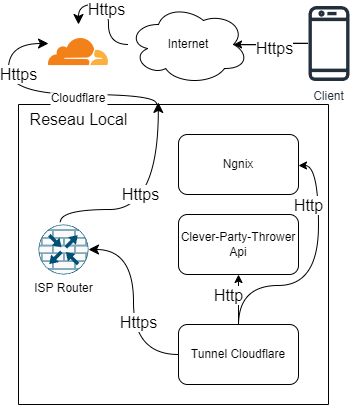
\includegraphics[width=\textwidth]{./images/shemaReseauDocker.drawio}
        \caption{Schema reseau Logique avec Docker}
        \label{fig:schemaDocker}
    \end{subfigure}
    \hfill
    \begin{subfigure}[b]{0.45\textwidth}
        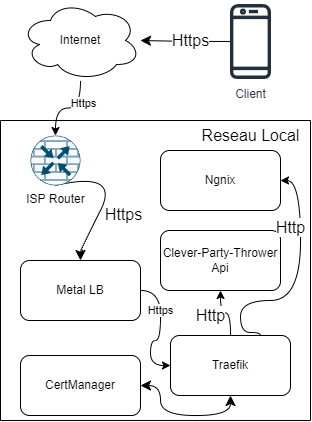
\includegraphics[width=\textwidth]{./images/shemaReseauKube.drawio}
        \caption{Schema reseau Logique avec Kubernetes}
        \label{fig:schemaKube}
    \end{subfigure}
    \caption{Le sens des differentes flèches représente le sens d'initialisation des connections}
    \label{fig:schemaReseau}
\end{figure}